\documentclass[a4paper,12pt]{article}
\usepackage{amsmath}
\usepackage{amsfonts}
\usepackage{amssymb}
\usepackage{graphicx}
\usepackage{url}
\usepackage{hyperref}
\usepackage{verbatim}
\usepackage{caption}
\usepackage{subcaption}


\title{Deathnote challenge}
\author{p3dr0ck}
\date{\today}

\newcommand{\challengeName}{deathnote}
\newcommand{\ip}{192.168.56.102}


\begin{document}

\maketitle


\noindent\textbf{Challenge Name}: \challengeName

\noindent\textbf{Link}: \href{https://www.vulnhub.com/entry/deathnote-1,739/}{The Vulnhub location is here}

\noindent\textbf{Description}: 
Level - easy
don't waste too much time thinking outside the box . It is a Straight forward box .
This works better with VirtualBox rather than VMware


\newpage


\section*{Solution}
Initially imported the machine OVA file in VirtualBox. 
In VirtualBox created a HostOnly network (192.168.56.1).
Then set the machine network interface to the HostOnlyAdapter (vboxnet0)

\begin{figure}[ht!]
	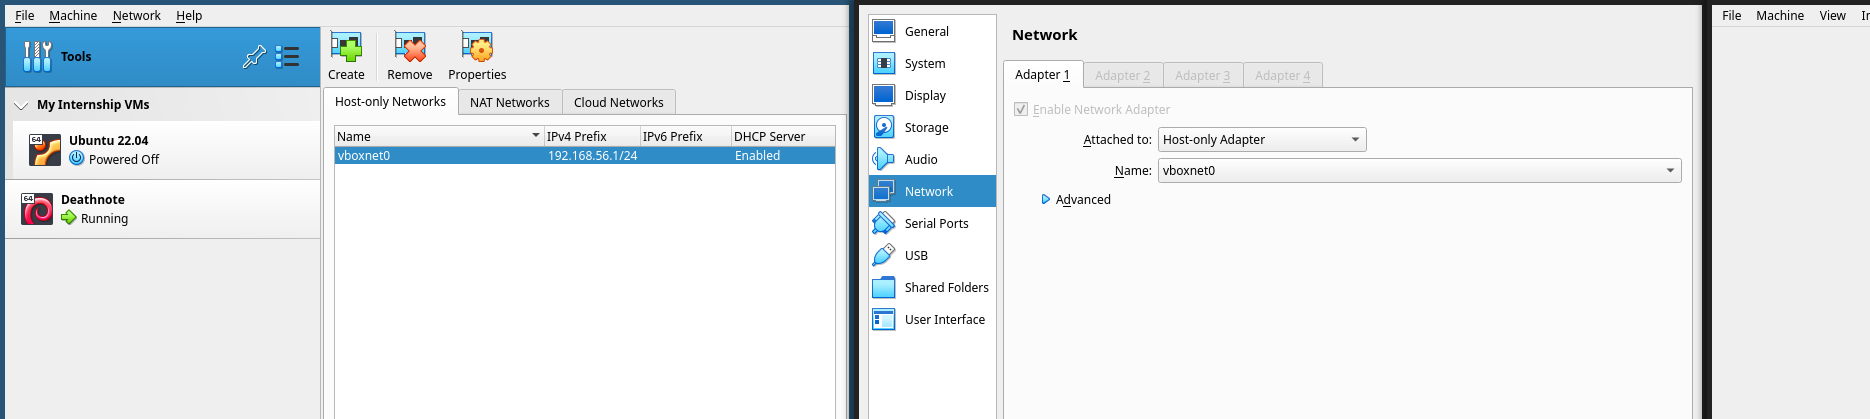
\includegraphics[width=\linewidth]{img/vbox_net_cfg.png}
	\caption{VirtualBox Network Setup}
	\label{fig:vbox_setup}
\end{figure}
 
 
After the bootup, pretty much nothing shows up, so started with a simple host-enumeration:
\begin{figure}[ht!]
	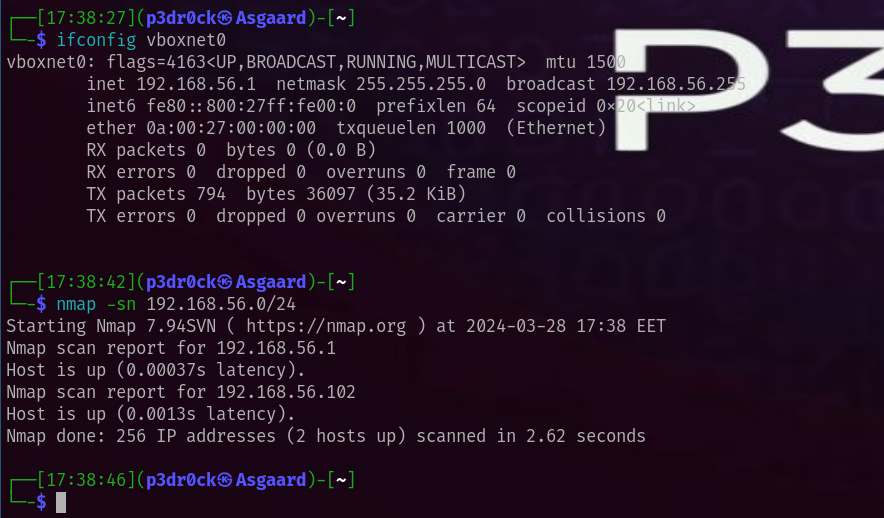
\includegraphics[width=\linewidth]{img/host_enumeration.png}
	\caption{Host Enumeration}
	\label{fig:host_enum}
\end{figure}

Next step, enumerate the ports
\begin{figure}[ht!]
	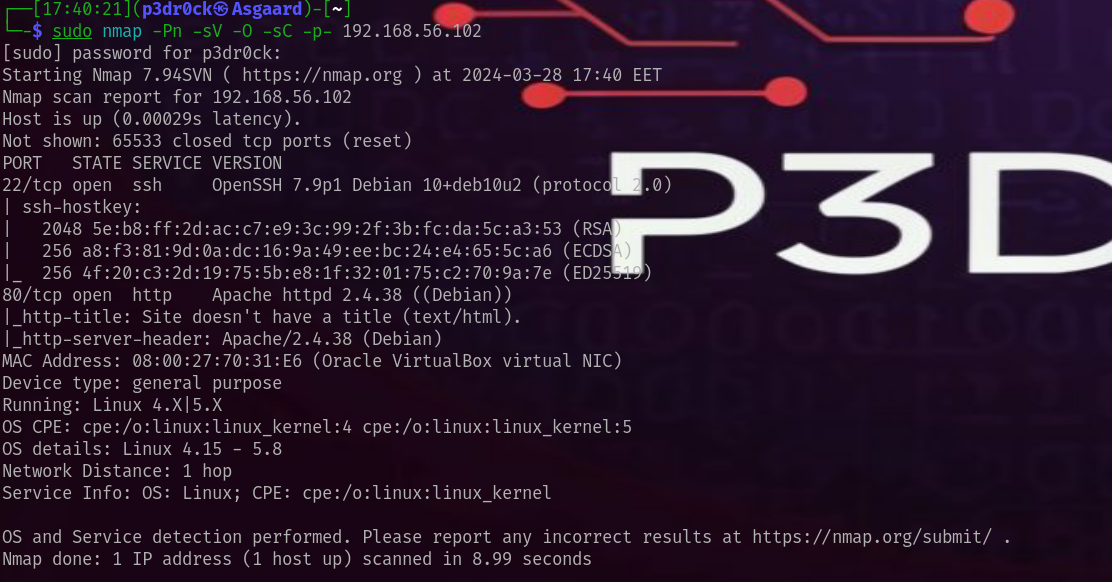
\includegraphics[width=\linewidth]{img/port_enumeration.png}
	\caption{Port Enumeration}
	\label{fig:port_enum}
\end{figure}

\subsection*{HTTP}
Decided to go forward with the HTTP first.
Putting the IP address into the browser \ip, will result in a redirect to the deathnote.vuln.
Thus decided to add the:
\begin{verbatim}
192.168.56.102 deathnote.vuln
\end{verbatim}
entry to the \textbf{/etc/hosts} file, to ease my life a bit.


Refreshing the browser it ends up showing the inial Figure \ref{fig:homepage} of the wordpress stuff.
\begin{figure}[t]
	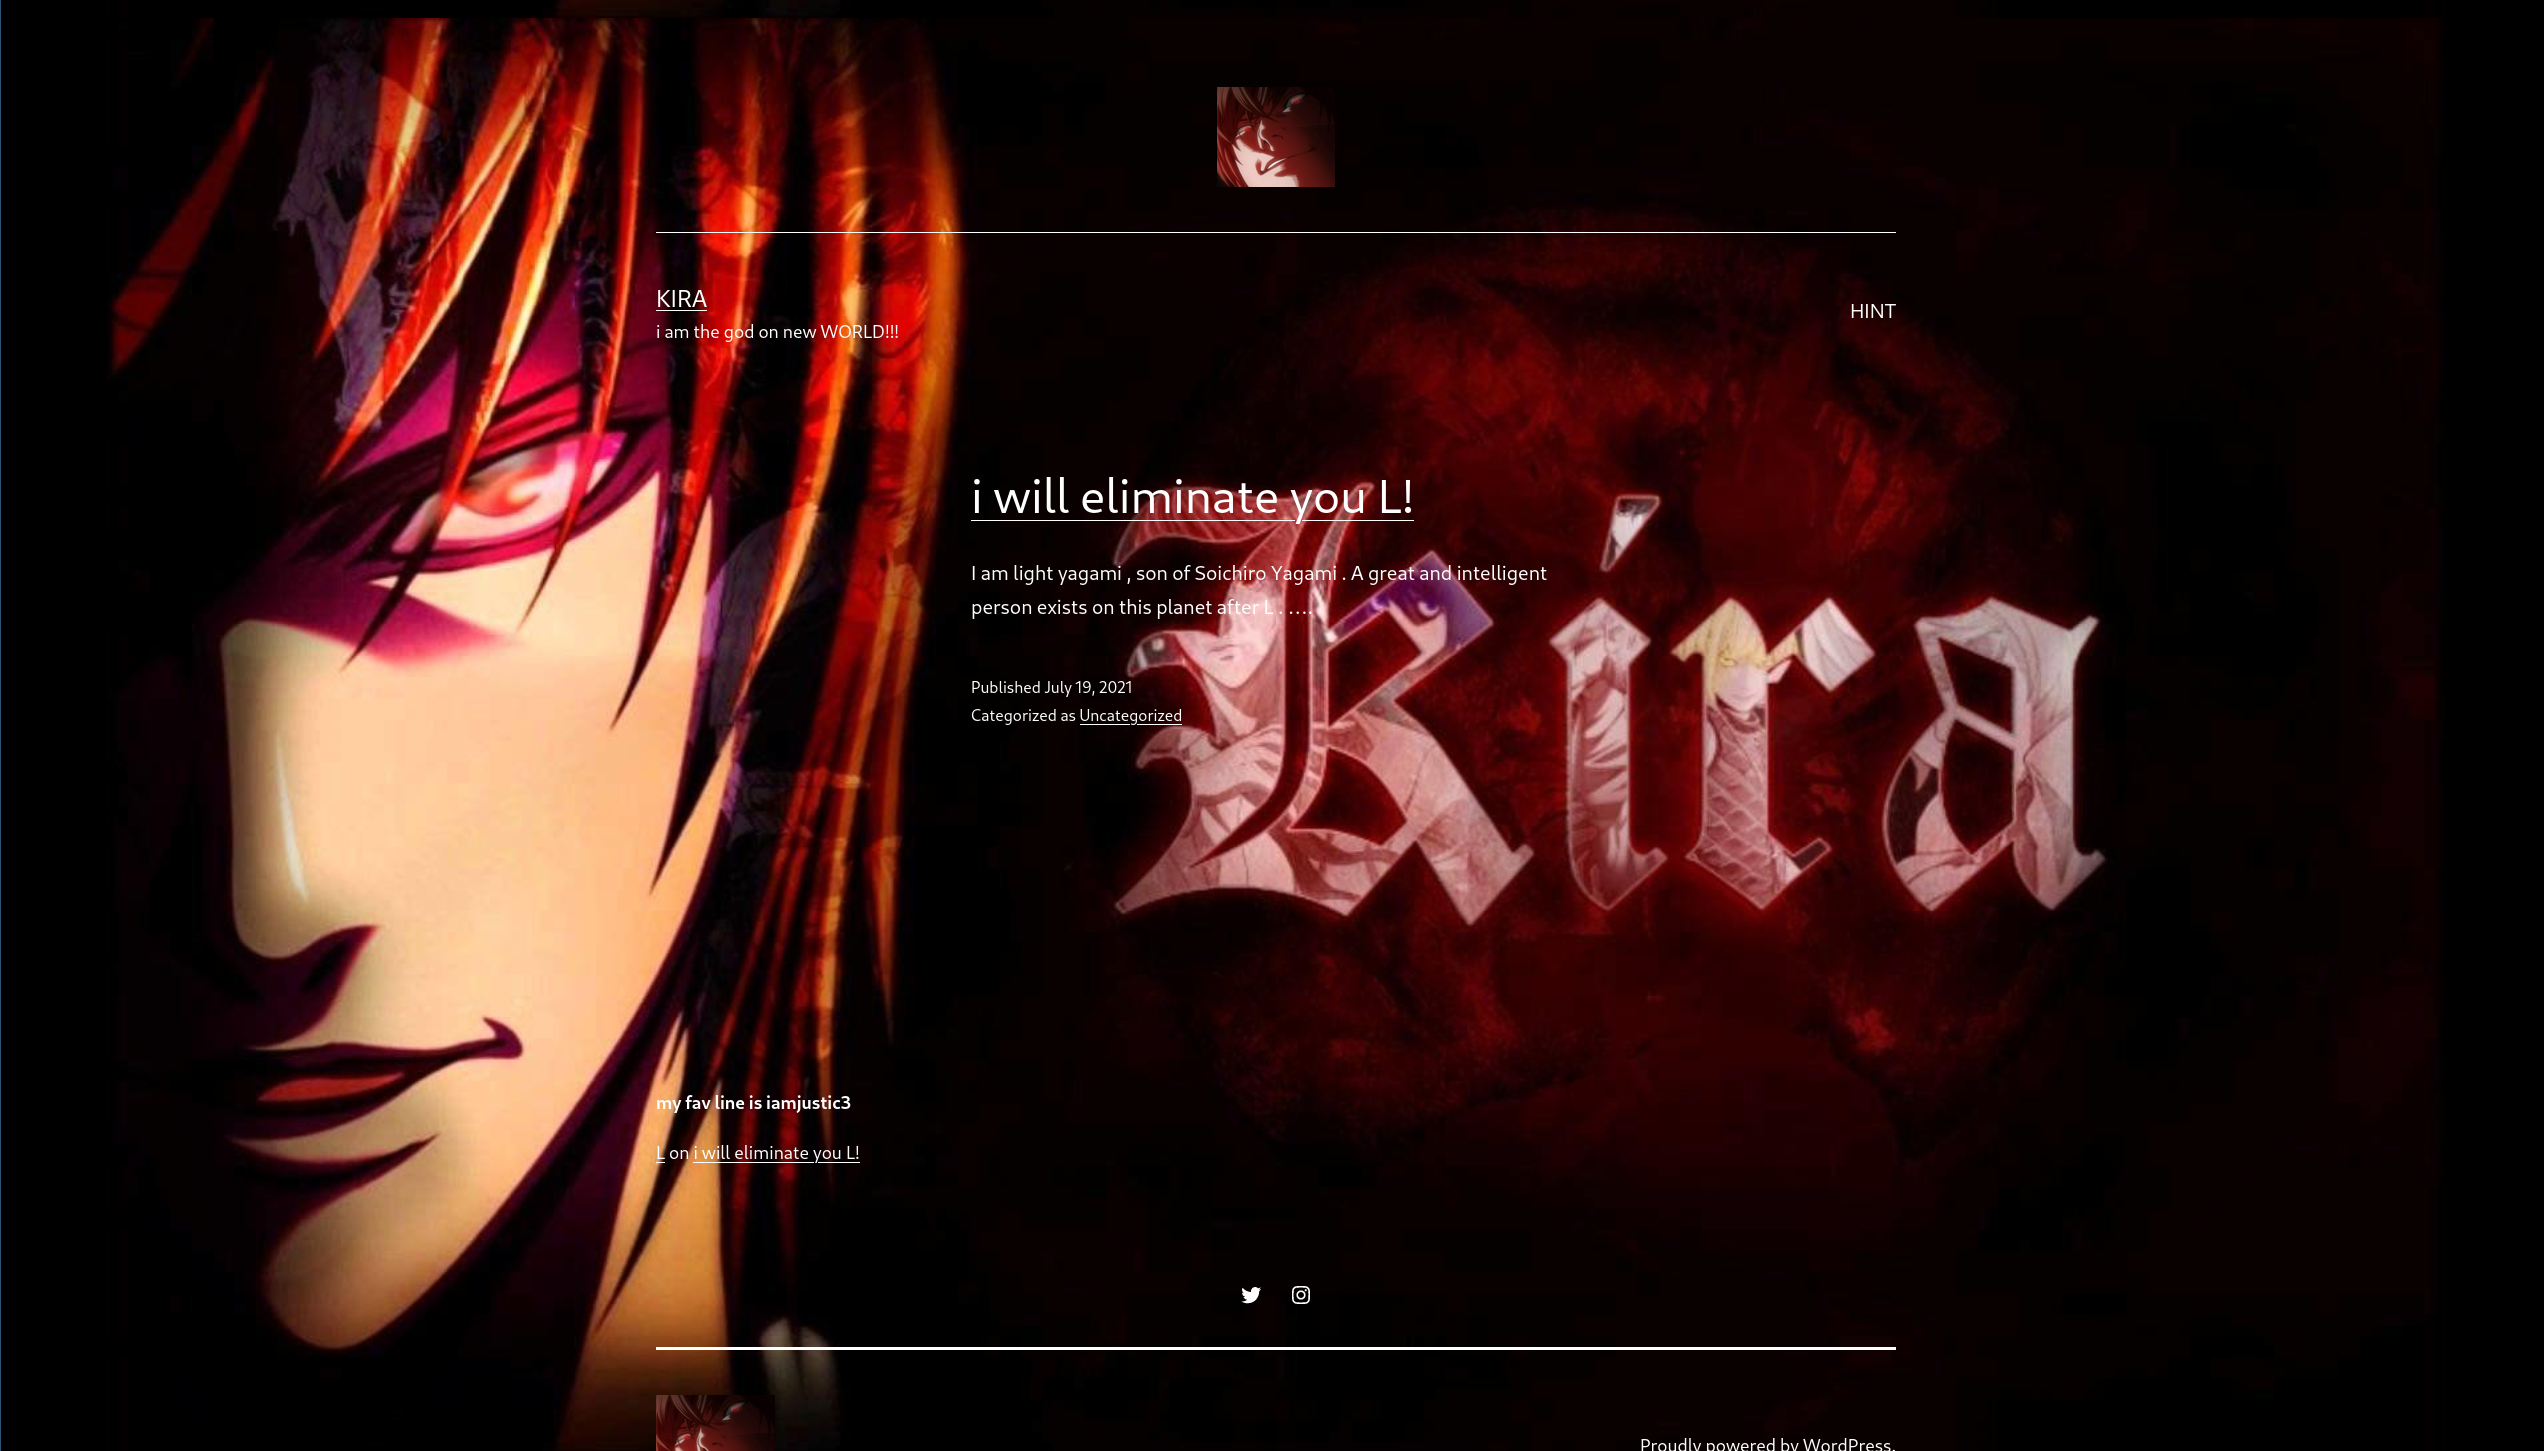
\includegraphics[width=\linewidth]{img/browser_00.png}
	\caption{Homepage}
	\label{fig:homepage}
\end{figure}
Playing a bit around, at the \textit{Hint} section is mentioned that:
\begin{quotation}
Find a notes.txt file on server
or
SEE the L comment 
\end{quotation}

The comment of L is:
\begin{quote}
I am light yagami , son of Soichiro Yagami . A great and intelligent person exists on this planet after L . ….
\end{quote}

So, decided to go with finding the notes.txt, as suggested on the Hint...
Doing this, decided to run wpscan, to see what directories, vulnerabilities the installed wordpress might have.

\newpage
\begin{minipage}[b]{\linewidth}
\scriptsize
\begin{verbatim}


[+] URL: http://192.168.56.102/wordpress/ [192.168.56.102]
[+] Started: Thu Mar 28 19:02:25 2024

Interesting Finding(s):

[+] Headers
 | Interesting Entry: Server: Apache/2.4.38 (Debian)
 | Found By: Headers (Passive Detection)
 | Confidence: 100%

[+] XML-RPC seems to be enabled: http://192.168.56.102/wordpress/xmlrpc.php
 | Found By: Direct Access (Aggressive Detection)
 | Confidence: 100%
 | References:
 |  - http://codex.wordpress.org/XML-RPC_Pingback_API
 |  - https://www.rapid7.com/db/modules/auxiliary/scanner/http/wordpress_ghost_scanner/
 |  - https://www.rapid7.com/db/modules/auxiliary/dos/http/wordpress_xmlrpc_dos/
 |  - https://www.rapid7.com/db/modules/auxiliary/scanner/http/wordpress_xmlrpc_login/
 |  - https://www.rapid7.com/db/modules/auxiliary/scanner/http/wordpress_pingback_access/

[+] WordPress readme found: http://192.168.56.102/wordpress/readme.html
 | Found By: Direct Access (Aggressive Detection)
 | Confidence: 100%

[+] Upload directory has listing enabled: http://192.168.56.102/wordpress/wp-content/uploads/
 | Found By: Direct Access (Aggressive Detection)
 | Confidence: 100%

[+] The external WP-Cron seems to be enabled: http://192.168.56.102/wordpress/wp-cron.php
 | Found By: Direct Access (Aggressive Detection)
 | Confidence: 60%
 | References:
 |  - https://www.iplocation.net/defend-wordpress-from-ddos
 |  - https://github.com/wpscanteam/wpscan/issues/1299

[+] WordPress version 5.8 identified (Insecure, released on 2021-07-20).
 | Found By: Emoji Settings (Passive Detection)
 |  - http://192.168.56.102/wordpress/, Match: 'wp-includes\/js\/wp-emoji-release.min.js?ver=5.8'
 | Confirmed By: Meta Generator (Passive Detection)
 |  - http://192.168.56.102/wordpress/, Match: 'WordPress 5.8'

[i] The main theme could not be detected.


[i] No plugins Found.


[i] No Config Backups Found.

[!] No WPScan API Token given, as a result vulnerability data has not been output.
[!] You can get a free API token with 25 daily requests by registering at https://wpscan.com/register

[+] Finished: Thu Mar 28 19:02:27 2024
[+] Requests Done: 164
[+] Cached Requests: 4
[+] Data Sent: 44.853 KB
[+] Data Received: 92.996 KB
[+] Memory used: 228.496 MB
[+] Elapsed time: 00:00:01


\end{verbatim}
\end{minipage}

The interesting thing here, is the
\scriptsize
\begin{verbatim}
[+] Upload directory has listing enabled: http://192.168.56.102/wordpress/wp-content/uploads/
\end{verbatim}
\normalsize
line, which tells me that on the webpage the \textit{wp-content/uploads} directory has the listings enabled!!!
Let's check that out!

\begin{figure}[ht!]
     \centering
     \begin{subfigure}[b]{0.4\textwidth}
         \centering
         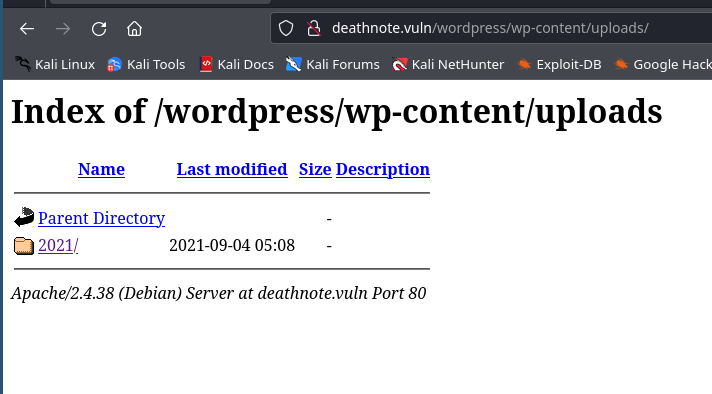
\includegraphics[width=\textwidth]{img/dirlist_00.png}
         \caption{Directory listing enabled!}
         \label{fig:dirlist}
     \end{subfigure}
     \hfill
     \begin{subfigure}[b]{0.4\textwidth}
         \centering
         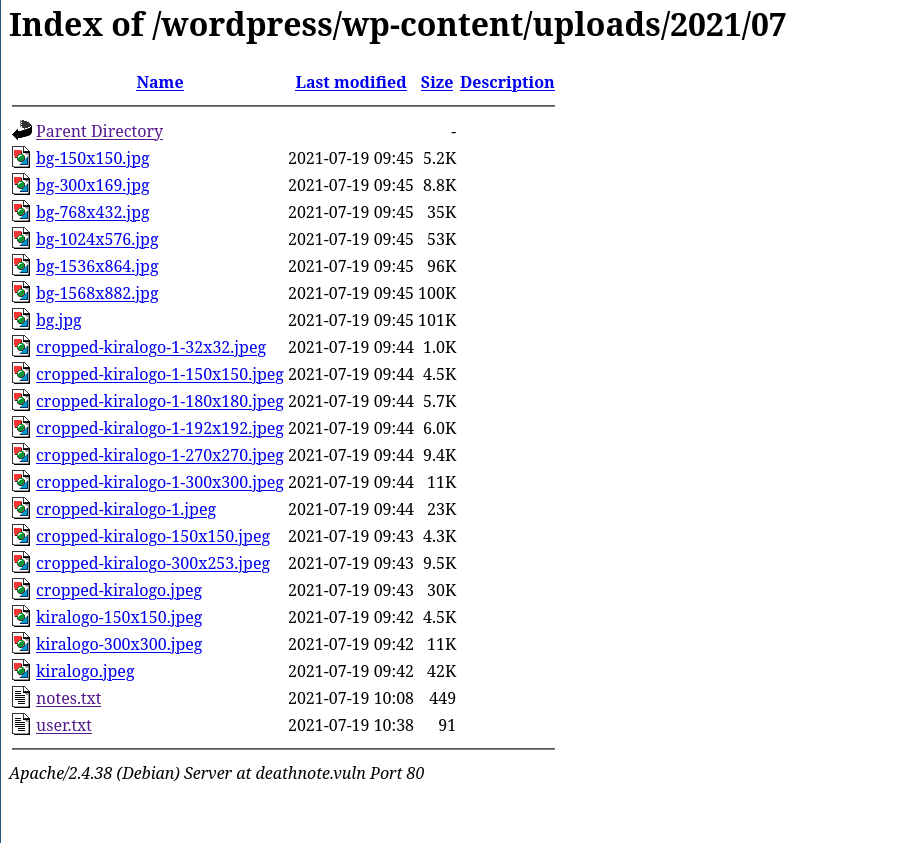
\includegraphics[width=\textwidth]{img/dirlist_01.png}
         \caption{Directory content!}
         \label{fig:dircontent}
     \end{subfigure}
     \caption{Direcotry listings}
     \label{fig:dirs}
\end{figure}

Indeed! Now, in the /wordpress/wp-content/uploads/2021/07 directory the notes.txt and user.txt files looks like some user/pass files. 
I think, maybe I can use them to login with ssh?


\subsection*{SSH}
Considering that we got a user list and a possible password list, the next logical step for me was to use
\textbf{hydra} to do a bruteforce attack on the ssh server.
\begin{verbatim}
hydra -L users.txt -P notes.txt 192.168.56.102 ssh
\end{verbatim}
Hydra finds a user/password combination which seems to work! 
\begin{itemize}
\item{user} \textbf{l}
\item{pass} \textbf{death4me}
\end{itemize}
Let's login!
\begin{figure}[ht!]
	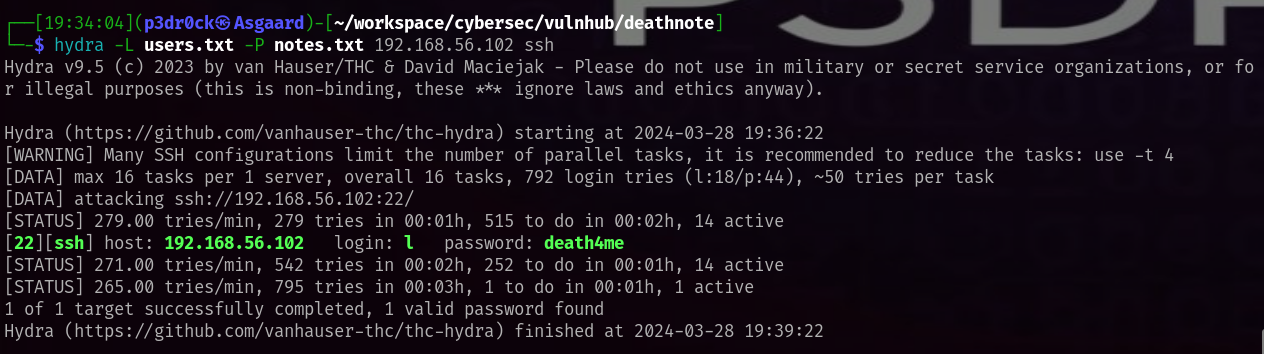
\includegraphics[width=\linewidth]{img/hydra.png}
	\caption{hydra}
	\label{fig:hydra}
\end{figure}


Logging in as user \textbf{l} is quick and easy. In it's home directory there is an user.txt file, which contains pretty much garbage.
Looking around, was able to chdir into user: \textit{kira}'s home directory.
Now, there is a file named kira.txt, with RWX permissions only for kira.
Exploring further, the .ssh directory of kira, doesn't have the correct access permissions!
I am able to looking into it, and an \verb|authorized_keys| file is found, which can be read by anybody! Looking into it, saw that it is an authorized key for the current l user! In kira's .ssh directory! It might let us in?
So, why not ssh to localhost, but this time with the kira username? And done!
We are kira now!
Now, we are able to read the kira.txt file in kira's home.

\scriptsize
\begin{verbatim}
kira@deathnote:~$ cat kira.txt 
cGxlYXNlIHByb3RlY3Qgb25lIG9mIHRoZSBmb2xsb3dpbmcgCjEuIEwgKC9vcHQpCjIuIE1pc2EgKC92YXIp
kira@deathnote:~$ cat kira.txt | base64 -d
please protect one of the following 
1. L (/opt)
2. Misa (/var)
\end{verbatim}
\normalsize

The next step is to look into those directories to see what we find.
In /var, pretty much standard stuff, thus, didn't wasted any time there.
\begin{figure}[ht!]
	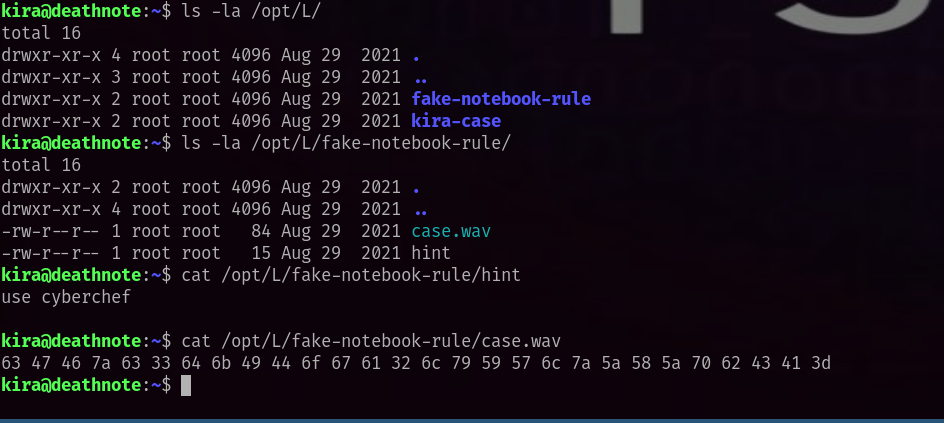
\includegraphics[width=\linewidth]{img/opt_00.png}
	\caption{opt}
	\label{fig:opt}
\end{figure}
As seen in \ref{fig:opt} the \textit{case.wav} file contains a list of hex characters. According to the \textit{hint} file, cyberchef is our friend to "decrypt" that.

\begin{figure}[ht!]
	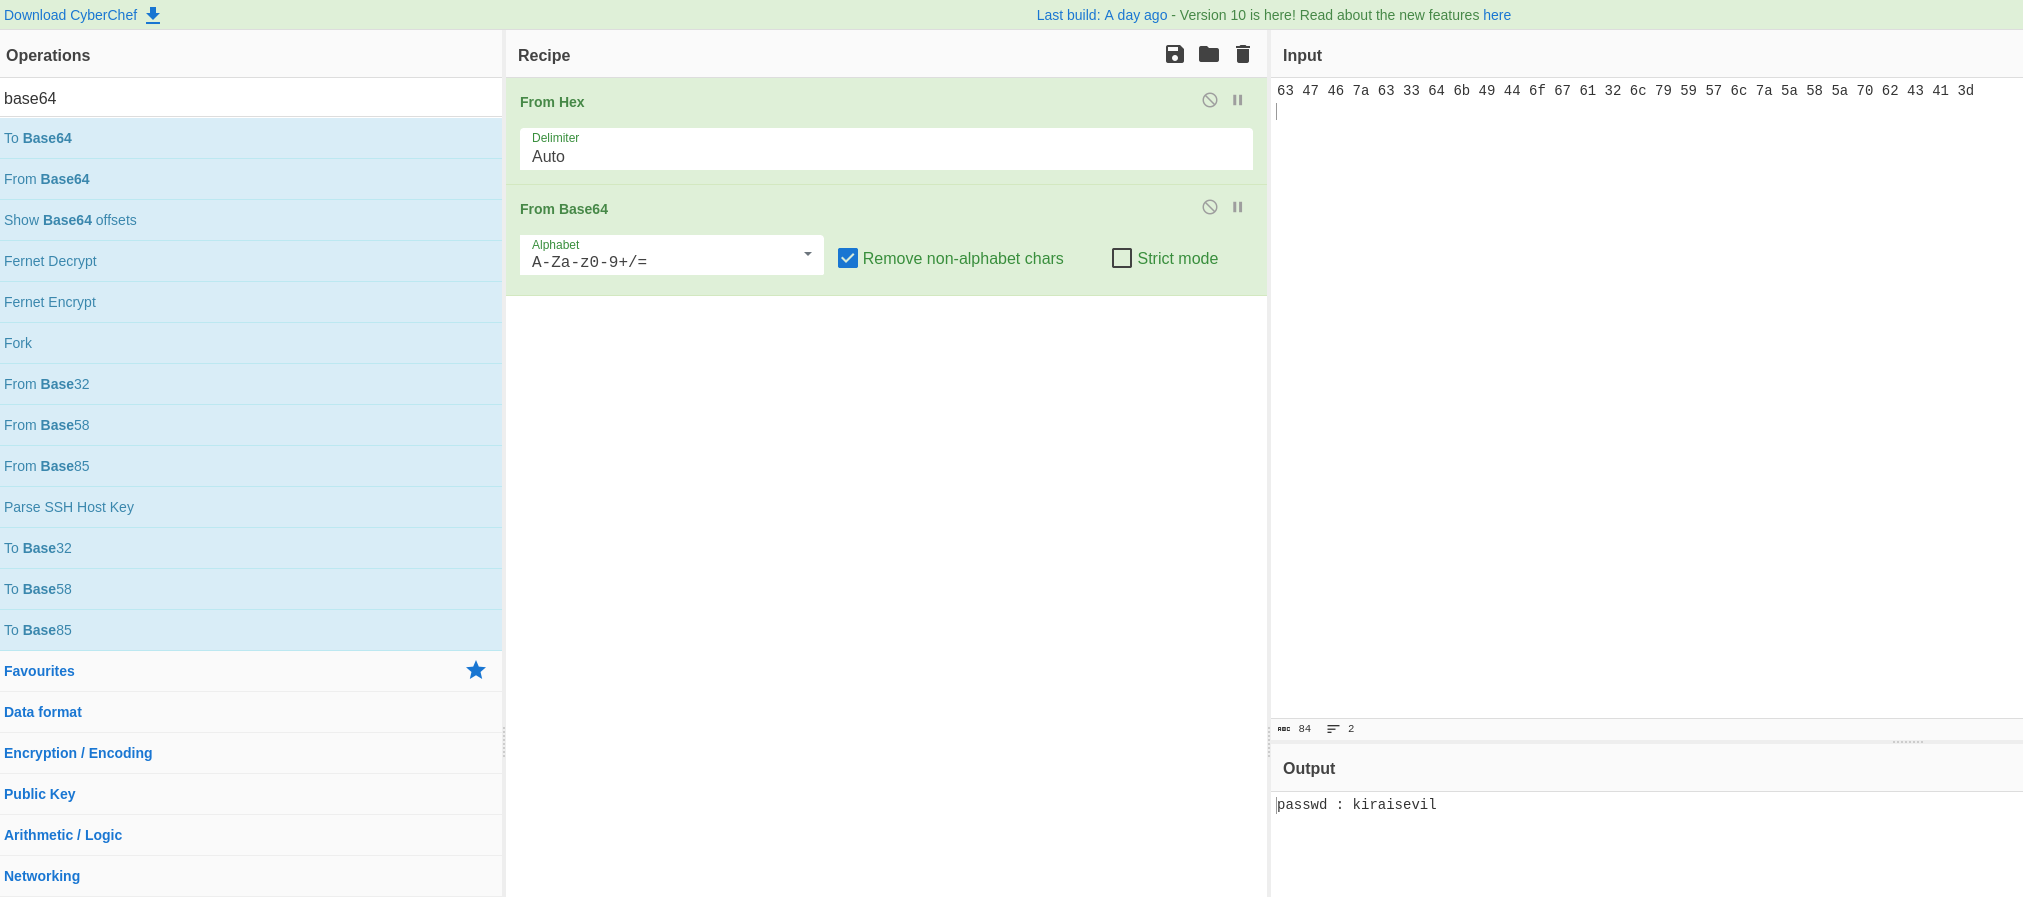
\includegraphics[width=\linewidth]{img/cyberchef.png}
	\caption{cyberchef}
	\label{fig:cyberchef}
\end{figure}

Using a hex to string, then a base64 decode, we got a password: \textbf{kiraisevil}.
At this stage, I used kira's credentials and logged in to the system.
Hitting the \textbf{id} command, I observed that kira has sudo rights, so did a \textbf{sudo su}.
Good. Now I',m not kira anymore, I'm root!
Rapidly chdir to root's home, then cat the \textit{root.txt} file, and I finished the machine!

\begin{figure}[ht!]
	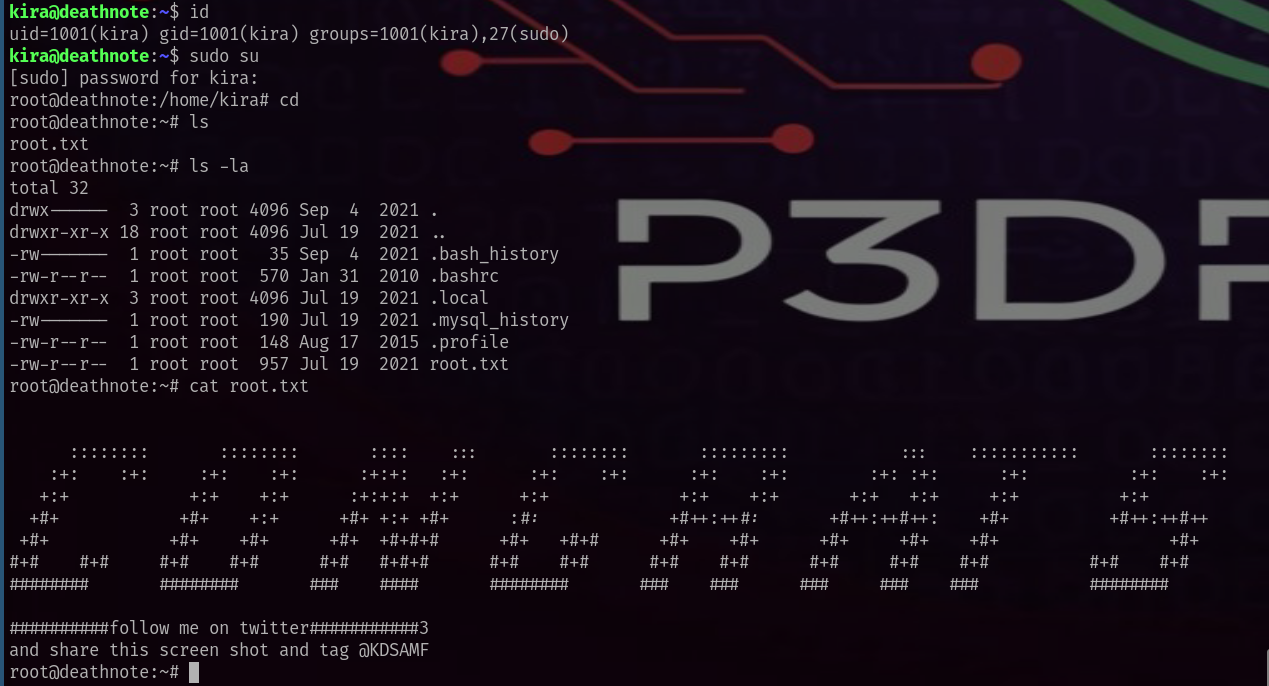
\includegraphics[width=\linewidth]{img/root.png}
	\caption{root}
	\label{fig:root}
\end{figure}



\end{document}
